\documentclass[a4j,10pt, twocolumn]{jarticle} \usepackage[dvipdfmx]{graphicx} \usepackage{amssymb} \usepackage{amsmath}
\usepackage{float}


\usepackage[compact]{titlesec}
\usepackage{fancyhdr}
\usepackage[dvipdfmx]{graphicx}
\usepackage[dvipdfmx]{color}

%---------------------------------------------------
% ページの設定
%---------------------------------------------------
\setlength{\textwidth}{179truemm}
\setlength{\textheight}{260truemm}
\setlength{\topmargin}{-14.5truemm}
\setlength{\oddsidemargin}{-9.5truemm}
\pagestyle{fancy}
\fancyhf{}
\fancyhead[L]{}
\fancyhead[C]{}
\fancyhead[R]{}
\renewcommand{\headrulewidth}{0pt}
\fancyfoot[L]{}
\fancyfoot[C]{}
\fancyfoot[R]{}
\renewcommand{\footrulewidth}{0pt}
\setlength{\headheight}{4truemm}
\setlength{\parindent}{1zw}


\begin{document}
\twocolumn
[
\begin{center}
  {\huge NAISTにて取り組みたい研究について}
\end{center}
\vspace{5truemm}
]

\rhead{
  \small{
  氏名: \rule{15mm}{3mm}, \
  試験区分: 情報科学区分, \
  希望研究室: 自然言語処理研究室, \ 
  現在の専門: 社会言語学
  }
}

\section{はじめに}
\subsection{NAISTで取り組みたいこと}
奈良先端科学技術大学院大学で取り組みたい研究テーマは「文脈を考慮した日本語の単語分散表現に存在するバイアスの緩和と評価」である。本稿では、研究テーマの研究背景・課題、研究方法、予想される結果、研究の特色、これまでの修学内容について述べる。

\section{研究の概要}
\subsection{研究の背景・課題}
単語分散表現とは、単語の意味をベクトル空間内で表現することである。様々な言語システムの基盤技術として広く使用されている。word2vecといった従来の分散表現に加え、文脈を考慮した分散表現として、BERTなどの汎用言語モデルも使用されるようになった。

word2vecやBERTといった分散表現では、意味が近いほど空間内の距離も近くなるようにベクトルが決定される。その際に使用する訓練データは、人間の社会的ステレオタイプが含まれるwebなどから取得しており、分散表現内へのバイアスの反映や増幅が起こる。実際に分散表現では、コンピュータサイエンスの関連用語を女性より男性の名前に近づけることがある。図1のように「cmu computer science phd student」と検索した場合、男性のwebページの方が検索結果の上位に掲載され、女性が見つかりにくくなってしまう\cite{Bolukbasi}。
\begin{figure}[ht]
    \centering
    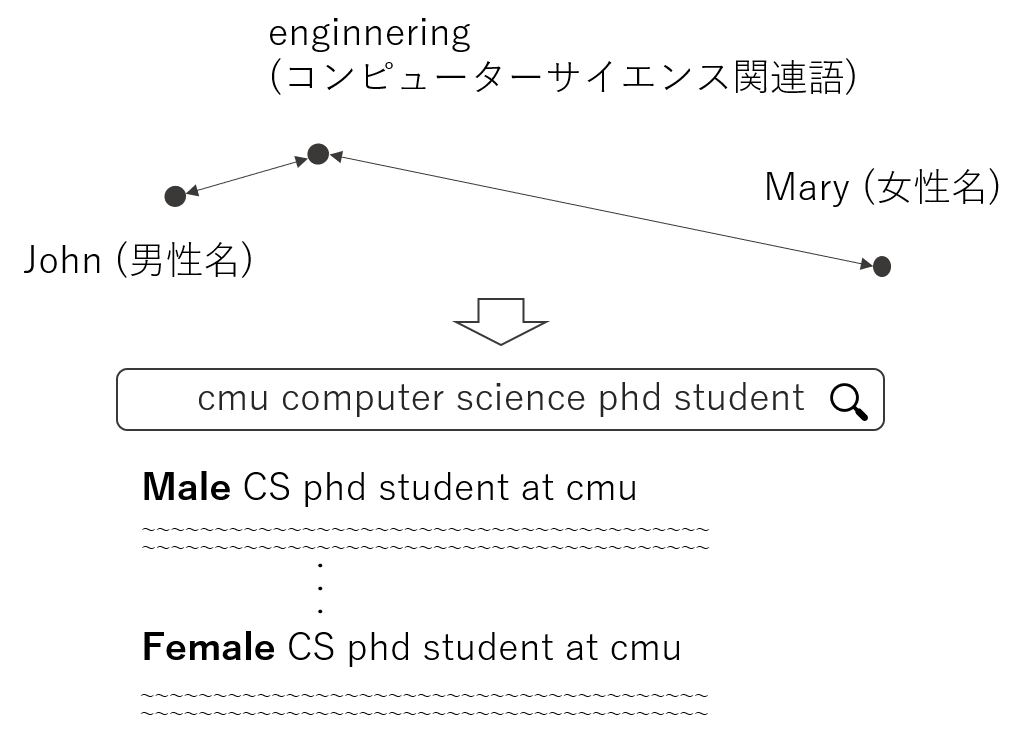
\includegraphics[width=70mm]{./bias_in_web.png}
    \caption{バイアスのあるベクトル空間とバイアスが反映されたweb検索結果画面}
\end{figure}

昨今、バイアスの分析や緩和に関する研究が行われている。
Bolukbashiらは、she-heやmale-femaleなどの定義的に性別が定まっているベクトルを使用してジェンダー方向を定め、programmerなどの職業語からジェンダー方向を除去することで緩和を試みた\cite{Bolukbasi}。また、英語のBERTではバイアスの除去に成功し、様々な下流タスクへ精度を落とさず使用するための研究が行われている\cite{P P Liang}。

日本語をはじめとするインド・ヨーロッパ言語以外の分散表現のバイアス研究は、2020年頃に開始されたばかりである\cite{Takeshita}。日本語では竹下らが、一般的なバイアス分析・緩和手法を、日本語の文脈考慮なし分散表現に適用できるか調査した\cite{Takeshita}。

日本語BERTのバイアス緩和に関する研究は未だ少ないが、word2vecに匹敵するほど様々なタスクに使用される汎用性があるため、今後BERTを下流タスクに応用したり、言語システムに使用したりするにあたり、BERTのバイアス緩和は望まれると考えている。

本研究ではBERTといった文脈を考慮した日本語の単語分散表現内のジェンダーバイアスの緩和とその評価を試みる。

\subsection{研究方法}
研究方法は大きく2ステップに分けられる。まず、(1)分散表現内のバイアスを緩和する。次に、(2)バイアス緩和前と後の差を評価し、効果的に緩和できているか確認する。目標とする状況は以下の通りである。
\begin{enumerate}
   \item 職業語など本来ジェンダーが中立であるべき単語のみを緩和できている。
   \item boyやmotherなど定義的にジェンダーが決められている単語はジェンダーの表現を維持できている。
   \item ジェンダー以外の特徴は維持できている。
\end{enumerate}
\subsubsection{バイアスの緩和}
バイアスの緩和手法について述べる。BERTのバイアス緩和手法で成功している既存の手法DensRay\cite{Liang}を日本語に適用することから始める。DensRayとは、Dufterらが発表したジェンダー部分空間を特定する方法であり、同じグループ(例:男性グループ)の距離は小さく、異なるグループの距離は大きくなるように単語ベクトルを写像する直交行列を求める\cite{Dufter, Liang}。BERTのAttention Headと層に使用する。Dufterらは、BERTの事前学習済みモデルのbert-base-uncasedの代わりに、bert-base-multilingual-uncasedを使用した中国語のバイアス緩和でも同様の成果が出たと述べている。bert-base-multilingual-uncasedと東北大学の訓練済み日本語BERTモデルを日本語に使用し、英語や中国語と同様の結果が出るか調査する。

\subsubsection{バイアスの評価}
具体的な評価手法について述べる。まず、Bartlらの研究\cite{Bartl}を日本語に踏襲する。BERTはMasked Language Modelという人為的にマスクした単語がなにか文脈から当てるという手法で学習しているため、その特性を利用する。まず、(i)定義的にジェンダーが決まっている語(例:彼)と(ii)ジェンダー中立であるべき職業語(例:保育士)から成る、表1に示すようなテンプレート文(文1)(文2)(文3)を用意する。
%また表1に示すなマスクをかけた(文1)をオリジナルの文としたとき、(文2)のように(i)と(ii)の語をマスクした文、(文3)のように(i)の語のみをマスクした文をテンプレート文として用意する.
\begin{table}[h]
    \centering
    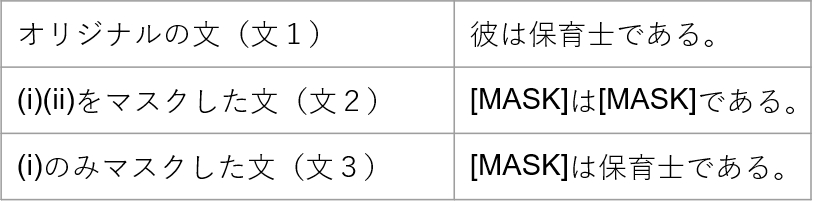
\includegraphics[width=75mm]{./processed_sentence.png}
    \caption{(i)(ii)をマスク処理した文と(i)のみ処理した文の例}
\end{table}

(文2)と(文3)をBERTに入力し、BERTが[MASK]を(i)と割り当てる確率をそれぞれ$p_{prior}$と$p_{tgt}$とする。$log\frac{P_{tgt}}{P_{prior}}$のように対数変換し、2つの確率の差を計算する。差が大きいほど(ii)に(i)のジェンダーが強く結びついていると考えられる。
バイアスの緩和前と緩和後のBERTモデルを比較する。緩和前に(ii)と強く結びついていたジェンダーは緩和後に軽減され、結びつきが弱かったジェンダーは増強され、結びつきの強さがどちらのジェンダーでも変わらなかった場合は維持されることを目標とする。
Bartlらの研究では、職業語のみで評価しているが、研究分野など他のカテゴリも使用することを検討している。また、モデル自体の性能が悪化していないかGLUEなどといった言語理解タスクで確認する必要がある。

\subsection{予想される結果}
DensRayの緩和手法は、表意文字の言語である中国語にも効果がある手法であるため、同じ表意文字の日本語にも使用できると期待できる。しかし、bert-base-multilingual-uncasedでは、トークナイズが日本語において適切ではないため\cite{Aoshima}、日本語では上手く緩和できない可能性がある。一方、東北大学の事前学習済みモデルは、文を形態素解析器MeCabでトークナイズしている。緩和対象は単語であることから、単語の意味を考慮せずにサブワードに分割するSentence Pieceなどと比べても、ジェンダー緩和に向いていると考えられ、英語や中国語と同様に緩和できると予想している。

Bartlは、提案したバイアス評価方法は、ドイツ語に適用できないと結論付けた\cite{Bartl}。ドイツ語は形態素が豊富で、名詞に男女の区別があり、動詞や形容詞、前置詞が名詞のジェンダーに合わせて変化することが原因として挙げられている。日本語は動詞や形容詞は活用するが、ドイツ語とは異なり名詞に男女の区別がないため、ドイツ語よりも正しく評価が可能と考えられる。

LeeはPronoun-drop言語の代表例に日本語を挙げている\cite{Lee}。Pronoun-drop言語とは、代名詞が推論可能な場合に省略される言語を指す。日本語と異なり、英語はpronoun-drop言語には該当しない。従って、BERTを学習する際、例えば「あの医者は娘と公園へ行った。その後、昼ご飯を食べた。」は英語だと"That doctor went to the park with his daughter. After that, he ate lunch."となり、"doctor"と"his"、"doctor"と"he"の関係を学習してしまう。一方、日本語では代名詞は省略され、それらの関係を学習しないため、BERTが保持しているバイアスが英語よりも弱い可能性がある。ただ、中国語も日本語ほど強くはないがPronoun-drop言語であるので、手法を試す余地はある。

\subsection{研究の特色}
近年、BLM運動やMeToo運動など、差別に抗議する活動が各地で起こり、差別の解消への気運が高まってきている。そういった中、自然言語処理技術のバイアスもより小さくなるよう向上させていくことは非常に重要となる。今後は英語のジェンダーバイアスだけでなく様々な言語・種類のバイアスに焦点を当てた研究を発展させていくことが望まれる。社会課題に直結した基盤技術を開発することで、現代社会が目指す理想像に寄り添うような言語処理システムを開発するための選択肢の一つを与えることができる。
%様々なシステムに応用が可能となり、社会にインパクトを与えられ

\section{これまでの修学内容等}
南山大学外国語学部フランス学科に在学している。言語学関連のゼミに所属しており、卒業論文として、人間の機械翻訳との関わり方について着手する予定である。

昨年度から東京都立大学小町研究室にて、基礎勉強会や論文紹介、ゼミなどに参加し、自然言語処理の研究に必要な基礎能力や基礎知識の習得を試みている。現在参加している基礎勉強会では、言語処理に関する機械学習・深層学習の書籍を輪読したり、単語分割プログラムや言語モデルなどの実装を行ったりしている。

\begin{thebibliography}{6}
{\footnotesize
\bibitem{Bolukbasi}
T. Bolukbasi et. al., "Man is to Computer Programmer as Woman is to Homemaker? Debiasing Word Embeddings," NIPS, 2016.
\bibitem{P P Liang}
P P Liang et. al., "Towards Debiasing Sentence Representations", ACL, 2020.
\bibitem{Takeshita}
M Takeshita et. al., "Can Existing Methods Debias Languages Other than English?
First Attempt to Analyze and Mitigate Japanese Word Embeddings," COLING, 2020.
\bibitem{Dufter}
P Dufter et. al., "Analytical Methods for Interpretable Ultradense Word Embeddings," EMNLP, 2019.
\bibitem{Liang}
S Liang et. al., "Monolingual and Multilingual Reduction of Gender Bias in Contextualized Representations," COLING, 2020.
\bibitem{Bartl}
M Bartl et. al., "Unmasking Contextual Stereotypes:
Measuring and Mitigating BERT’s Gender Bias," COLING, 2020.
\bibitem{Aoshima}
青嶋智久 et al., "日本語BERTモデルを用いた経済テキストテキストデータのセンチメント分析, " 人工知能学会全国大会, 2019.
\bibitem{Lee}
S Lee, "Rethinking the relationship between pronoun-drop and individualism with Bayesian multilevel models", Journal of Language Evolution, 2017
}
\end{thebibliography}
\end{document}